\begin{frame}\frametitle{Requirements for Selection of $W\gamma$ Candidates}
% ADD A PLOT WITH GEOMETRY (eta)
  \begin{table}[h]
     \tiny
     \begin{center}
     \begin{tabular}{|c|c|l|}
     \hline
     \multicolumn{2}{|c|}{\scriptsize{Selection requirements for candidates}} & {\scriptsize{Comment}} \\ 
     {\bfseries{- - - - - - $W\gamma\rightarrow\mu\nu\gamma$ - - - - - -}} & 
     {\bfseries{- - - - - - $W\gamma\rightarrow e\nu\gamma$ - - - - - -}}  & \\ \hline

    \multicolumn{2}{|c|}{\scriptsize\bfseries{Event level:}}  & \\ 
     \multicolumn{2}{|c|}{Exactly one lepton + at least one photon}  & process signature\\  
      \multicolumn{2}{|c|}{$M_T^W>$40~GeV} & rejects DY+jets, $Z\gamma$\\ 
                                & 110$>M_{e\gamma}>$70~GeV excl. & rejects DY+jets\\ 
      \multicolumn{2}{|c|}{$\Delta{R}(lep,\gamma)>$0.7} & theory consideration\\  \hline

     \multicolumn{2}{|c|}{\scriptsize\bfseries{Photon selection:}} & \\
     \multicolumn{2}{|c|}{\tiny{$P_T^{\gamma}>$15~GeV}} & theory considerations \\ 
     \multicolumn{2}{|c|}{\tiny{$\eta^{\gamma}$: EB or EE}} & acceptance \\ 
     \multicolumn{2}{|c|}{\tiny{Photon ID}} & POG*-recommended \\ 
             &{\tiny{ [one change in ID]}} & $W\gamma\gamma$-recommended\\ \hline

     \multicolumn{2}{|c|}{\scriptsize\bfseries{Lepton selection:}} & \\
      \tiny{$p_T^{\mu}>$25~GeV;} &  \tiny{$p_T^{e}>$30~GeV;}  & trigger\\ 
      \tiny{$|\eta^{\mu}|<2.1$} & \tiny{  $\eta^{e}$: EB or EE} & trigger, acceptance\\ 
      Muon ID & Electron ID & POG*-recommended \\ \hline

      \multicolumn{2}{|c|}{\scriptsize\bfseries{Second lepton veto:}} & rejects DY+jets, $Z\gamma$\\
      \tiny{$p_T^{\mu2}>10$ GeV;} &  \tiny{$p_T^{e2}>10$ GeV;} & \\
      \tiny{$|\eta^{\mu2}|<2.4$}  &   \tiny{ $\eta^{e2}$: EB or EE} &  \\
                                &   \tiny{[veto] ID} & very loose \\ \hline
      \end{tabular}
      \end{center}
  \end{table}
\scriptsize
If we have several candidates in an event, we choose one with the highest $P_T^{\gamma}$\\
-\\
\tiny
*POG - Particle Object Group (in CMS)\\
\end{frame}%{Event-Level Selection Requirements}

\begin{frame}\frametitle{Data vs MC. $M_T^W$ and $M_{l\gamma}$}
\scriptsize
{\bfseries{$M_T^W>40$~GeV}} is applied in both channels\\
{\bfseries{$M_{l,\gamma}<70~or~M_{l,\gamma}>110$~GeV}} is applied in the {\bfseries{electron channel}} only
\begin{figure}[htb]
  \begin{center}
   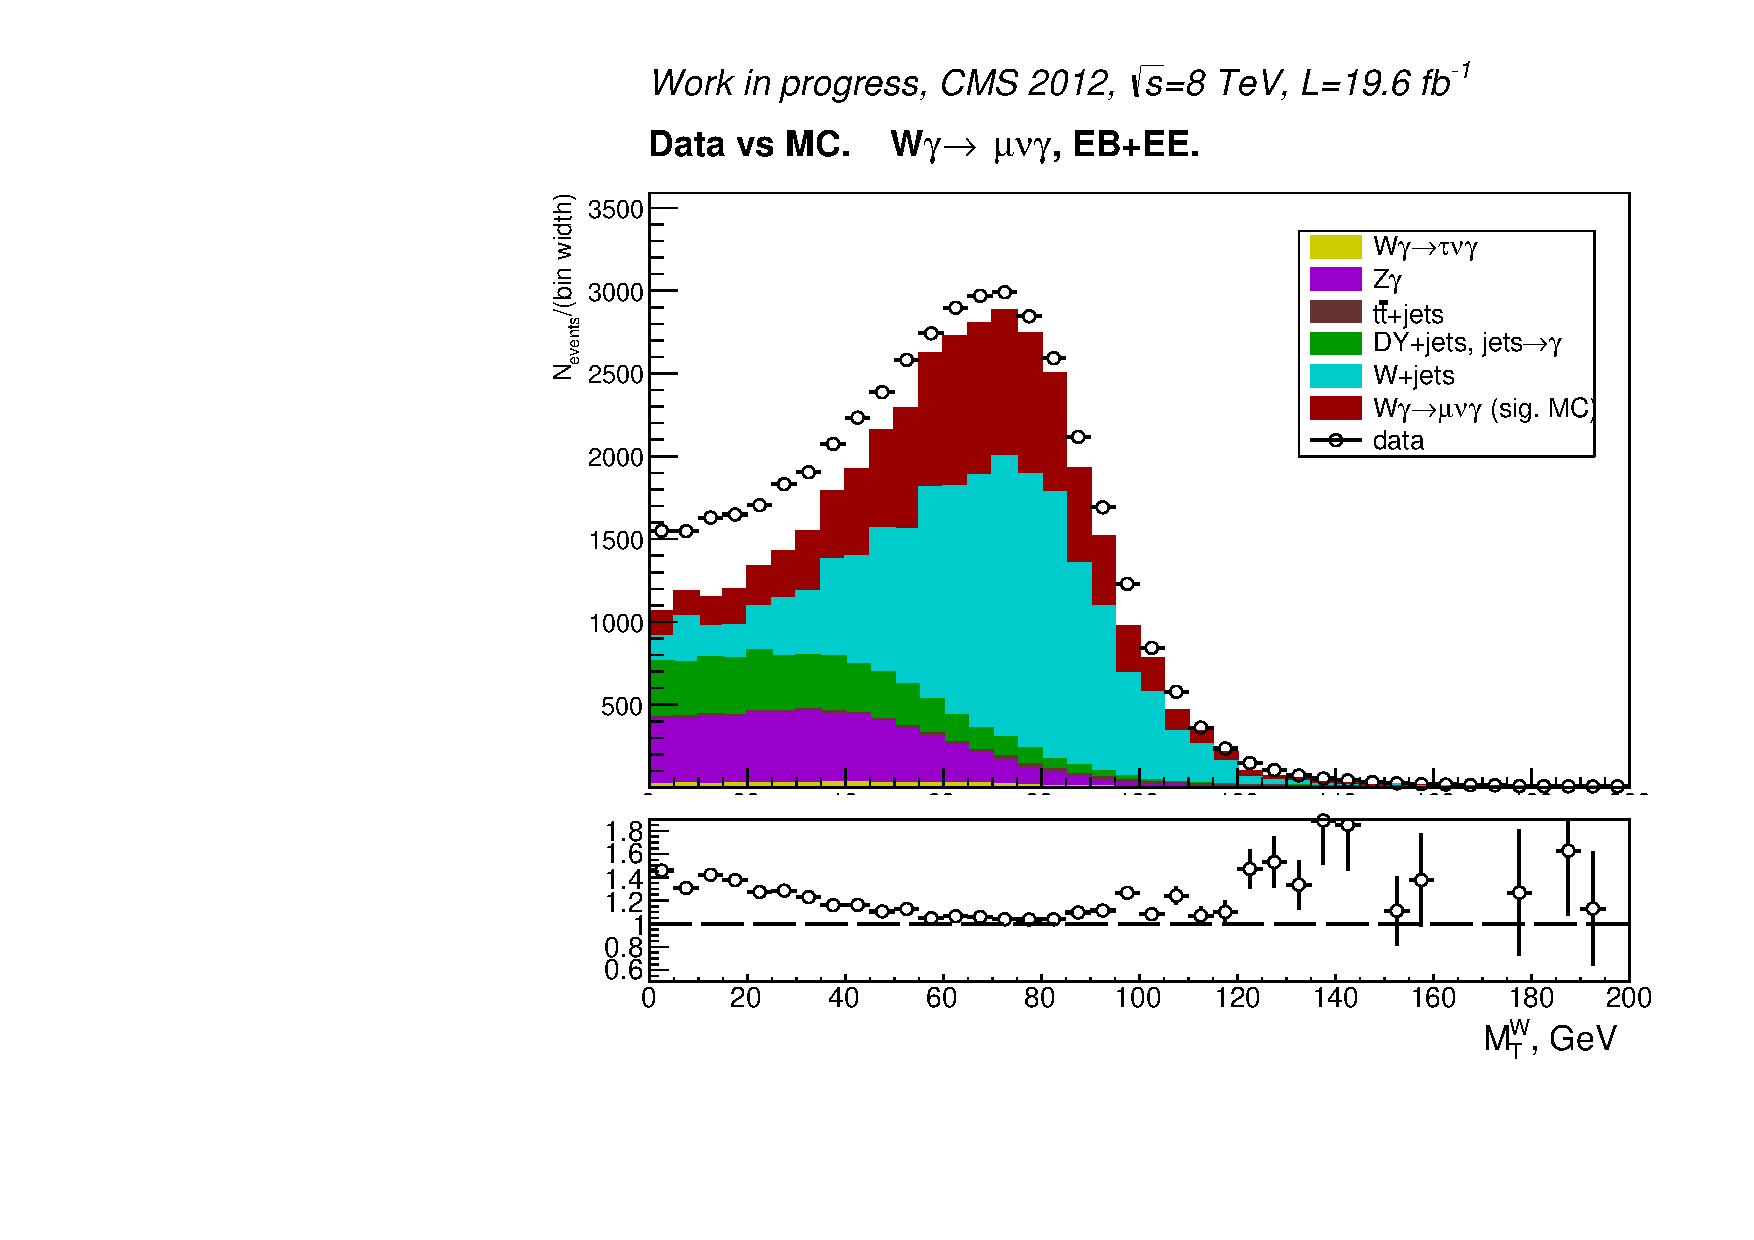
\includegraphics[width=0.33\textwidth]{../figs/figs_v11/MUON_WGamma/PrepareYields/c_TotalDATAvsMC_EtaCommon__WMtVERY_PRELIMINARY.pdf}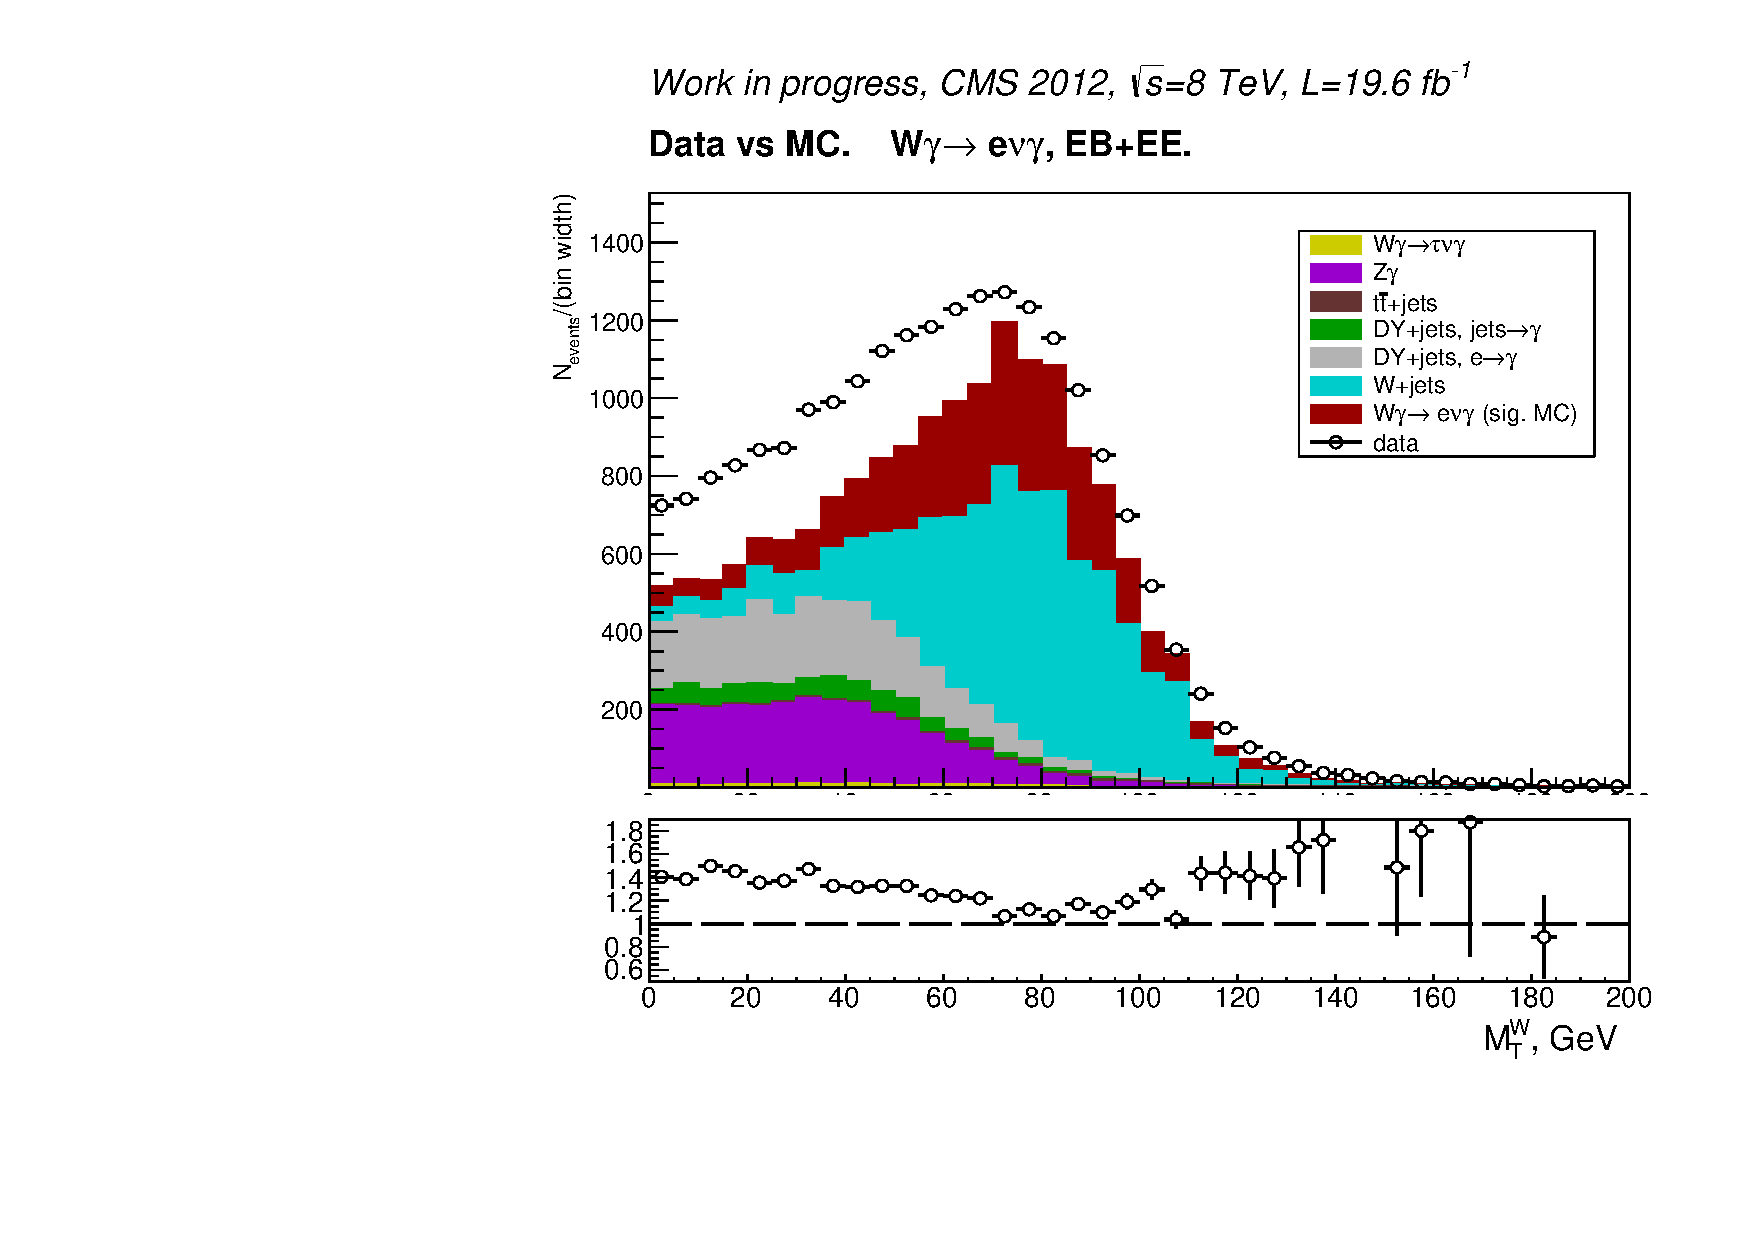
\includegraphics[width=0.33\textwidth]{../figs/figs_v11/ELECTRON_WGamma/PrepareYields/c_TotalDATAvsMC_EtaCommon__WMtVERY_PRELIMINARY.pdf}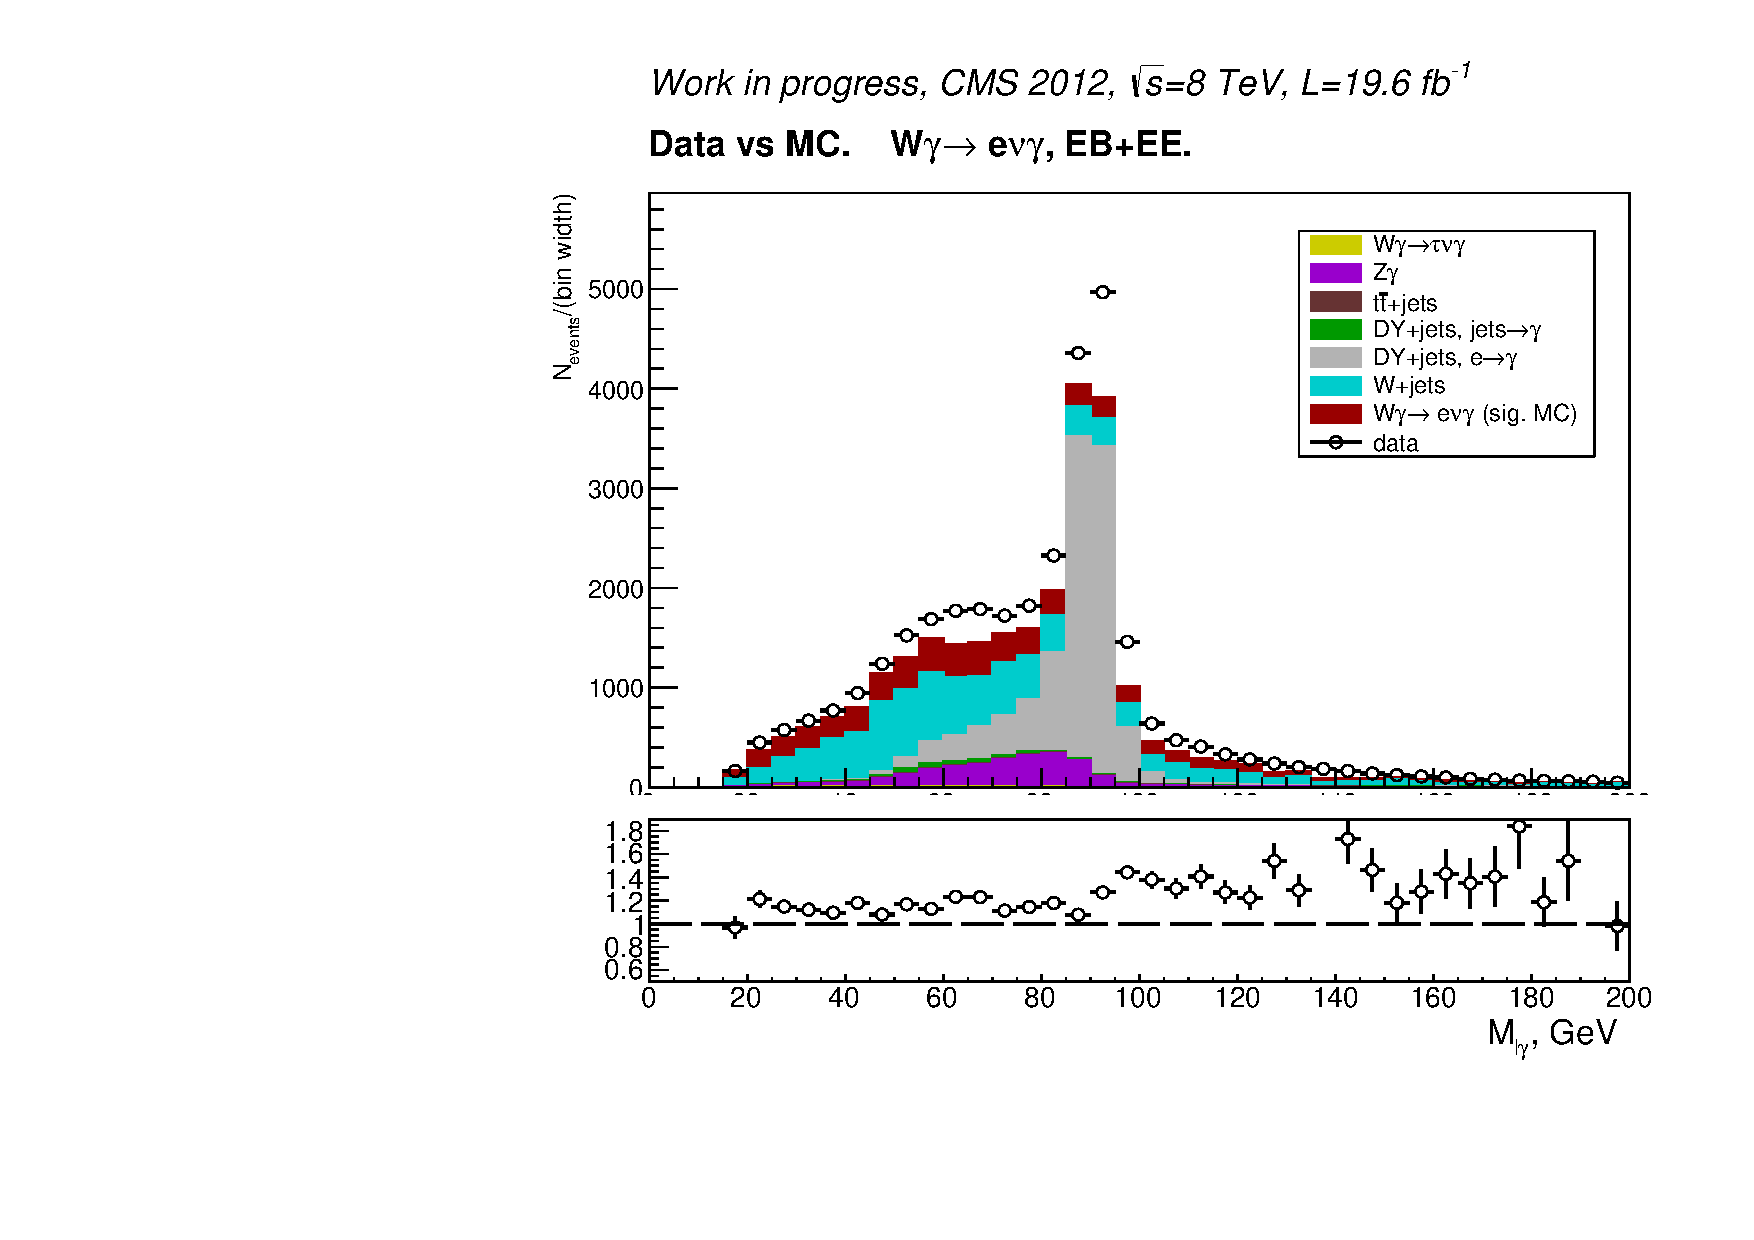
\includegraphics[width=0.33\textwidth]{../figs/figs_v11/ELECTRON_WGamma/PrepareYields/c_TotalDATAvsMC_EtaCommon__Mpholep1PRELIMINARY_FOR_E_TO_GAMMA_WITH_PSV_CUT.pdf}
  \end{center}
\end{figure}
\end{frame}

\begin{frame}\frametitle{Data vs MC. $P_T^{\gamma}$}
\scriptsize
\begin{itemize}
   \item Selected datasets are dominated by $W$+jets events in low $P_T^{\gamma}$ bins;
   \item Fraction of signal increases with $P_T^{\gamma}$;
   \item Data disagree with MC.
\end{itemize}
  \begin{figure}[htb]
    \begin{center}
       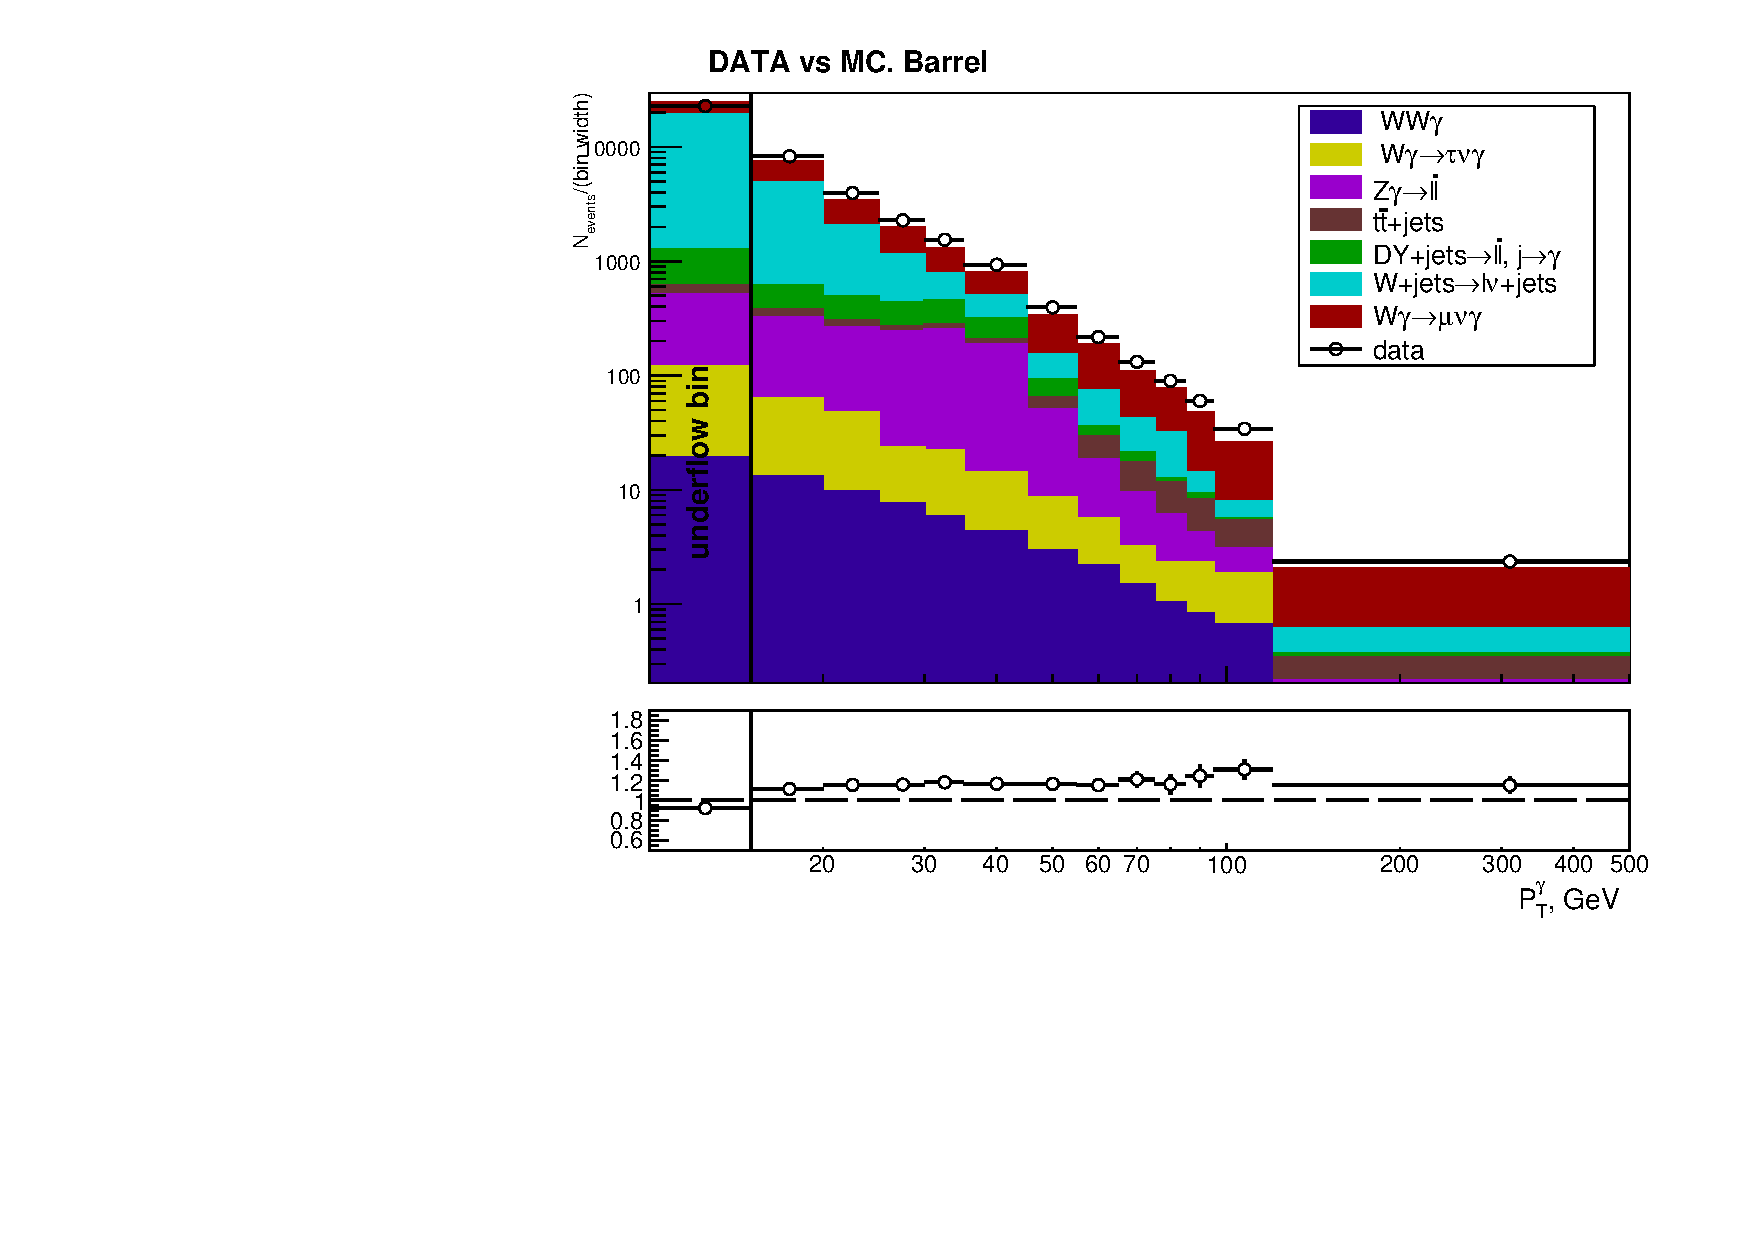
\includegraphics[width=0.49\textwidth]{../figs/figs_v11/MUON_WGamma/PrepareYields/c_TotalDATAvsMC_Barrel__phoEt.pdf} 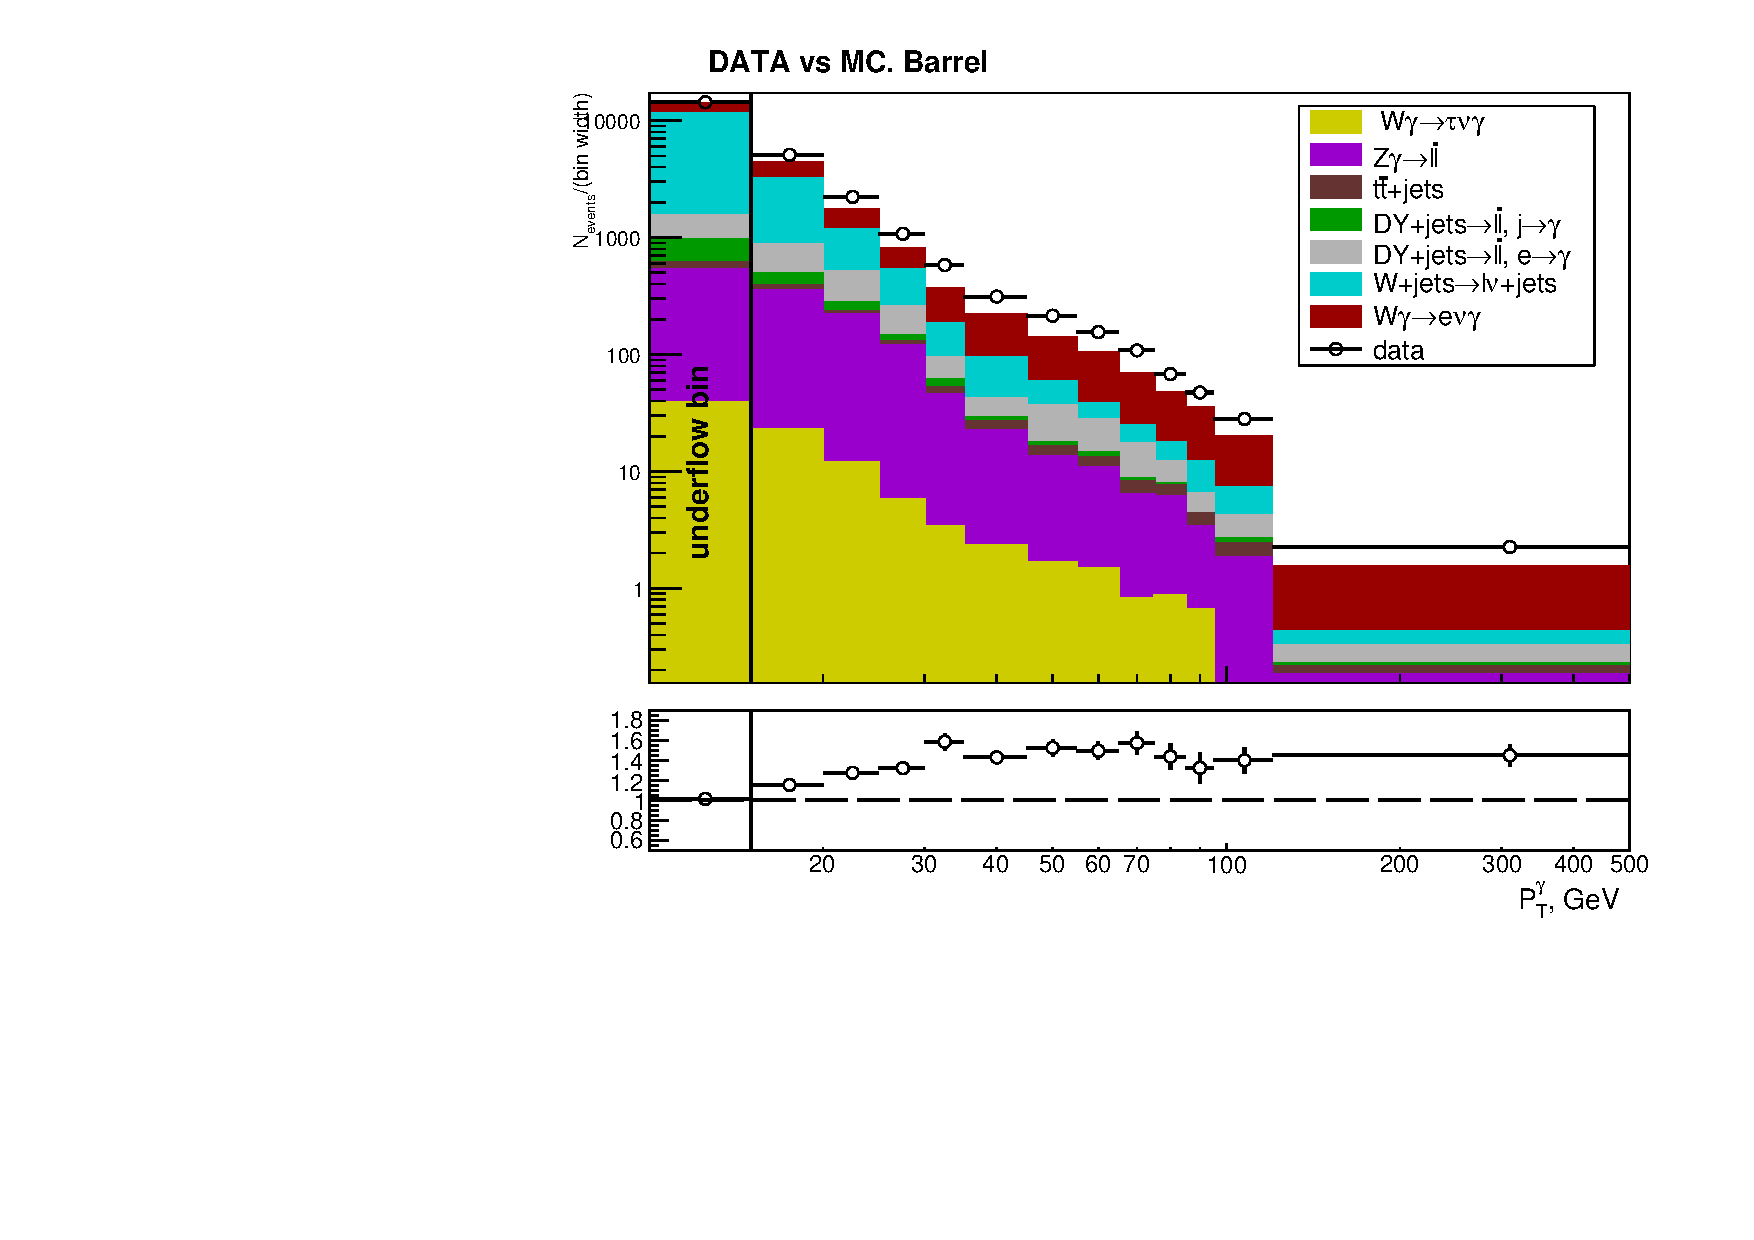
\includegraphics[width=0.49\textwidth]{../figs/figs_v11/ELECTRON_WGamma/PrepareYields/c_TotalDATAvsMC_Barrel__phoEt.pdf} 
    \end{center}
  \end{figure}
\tiny
All MC samples are normalized to the luminosity of data.
\end{frame}


\begin{frame}\frametitle{Data vs MC. $P_T^{\gamma}$}
\scriptsize
Backgrounds:
\begin{itemize}
   \item jets$\rightarrow\gamma$: $W$+jets, DY+jets, $t\bar{t}$+jets;
   \item $e\rightarrow\gamma$: DY+jets, electron channel only;
   \item real-$\gamma$: $Z\gamma$, $W\gamma\rightarrow\tau\nu\gamma$.
\end{itemize}
  \begin{figure}[htb]
    \begin{center}
       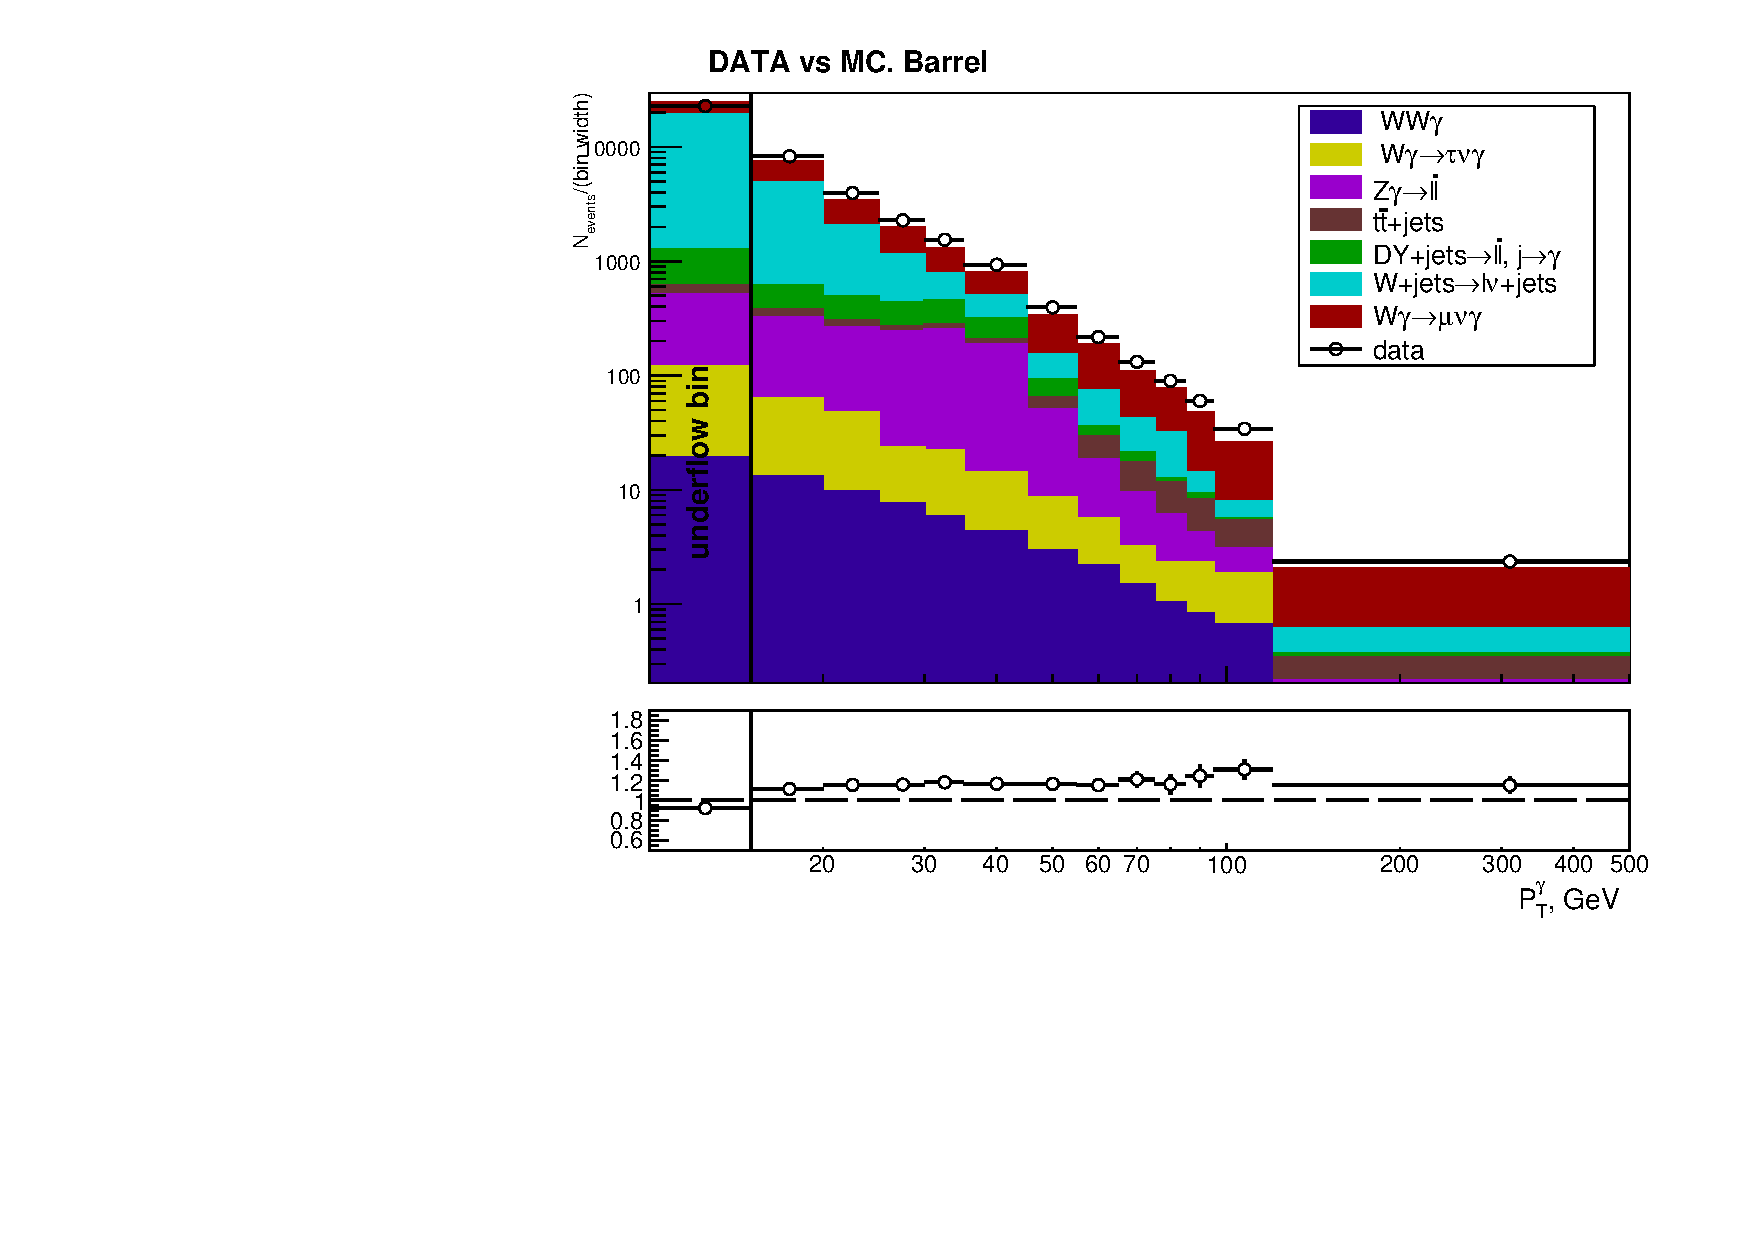
\includegraphics[width=0.49\textwidth]{../figs/figs_v11/MUON_WGamma/PrepareYields/c_TotalDATAvsMC_Barrel__phoEt.pdf} 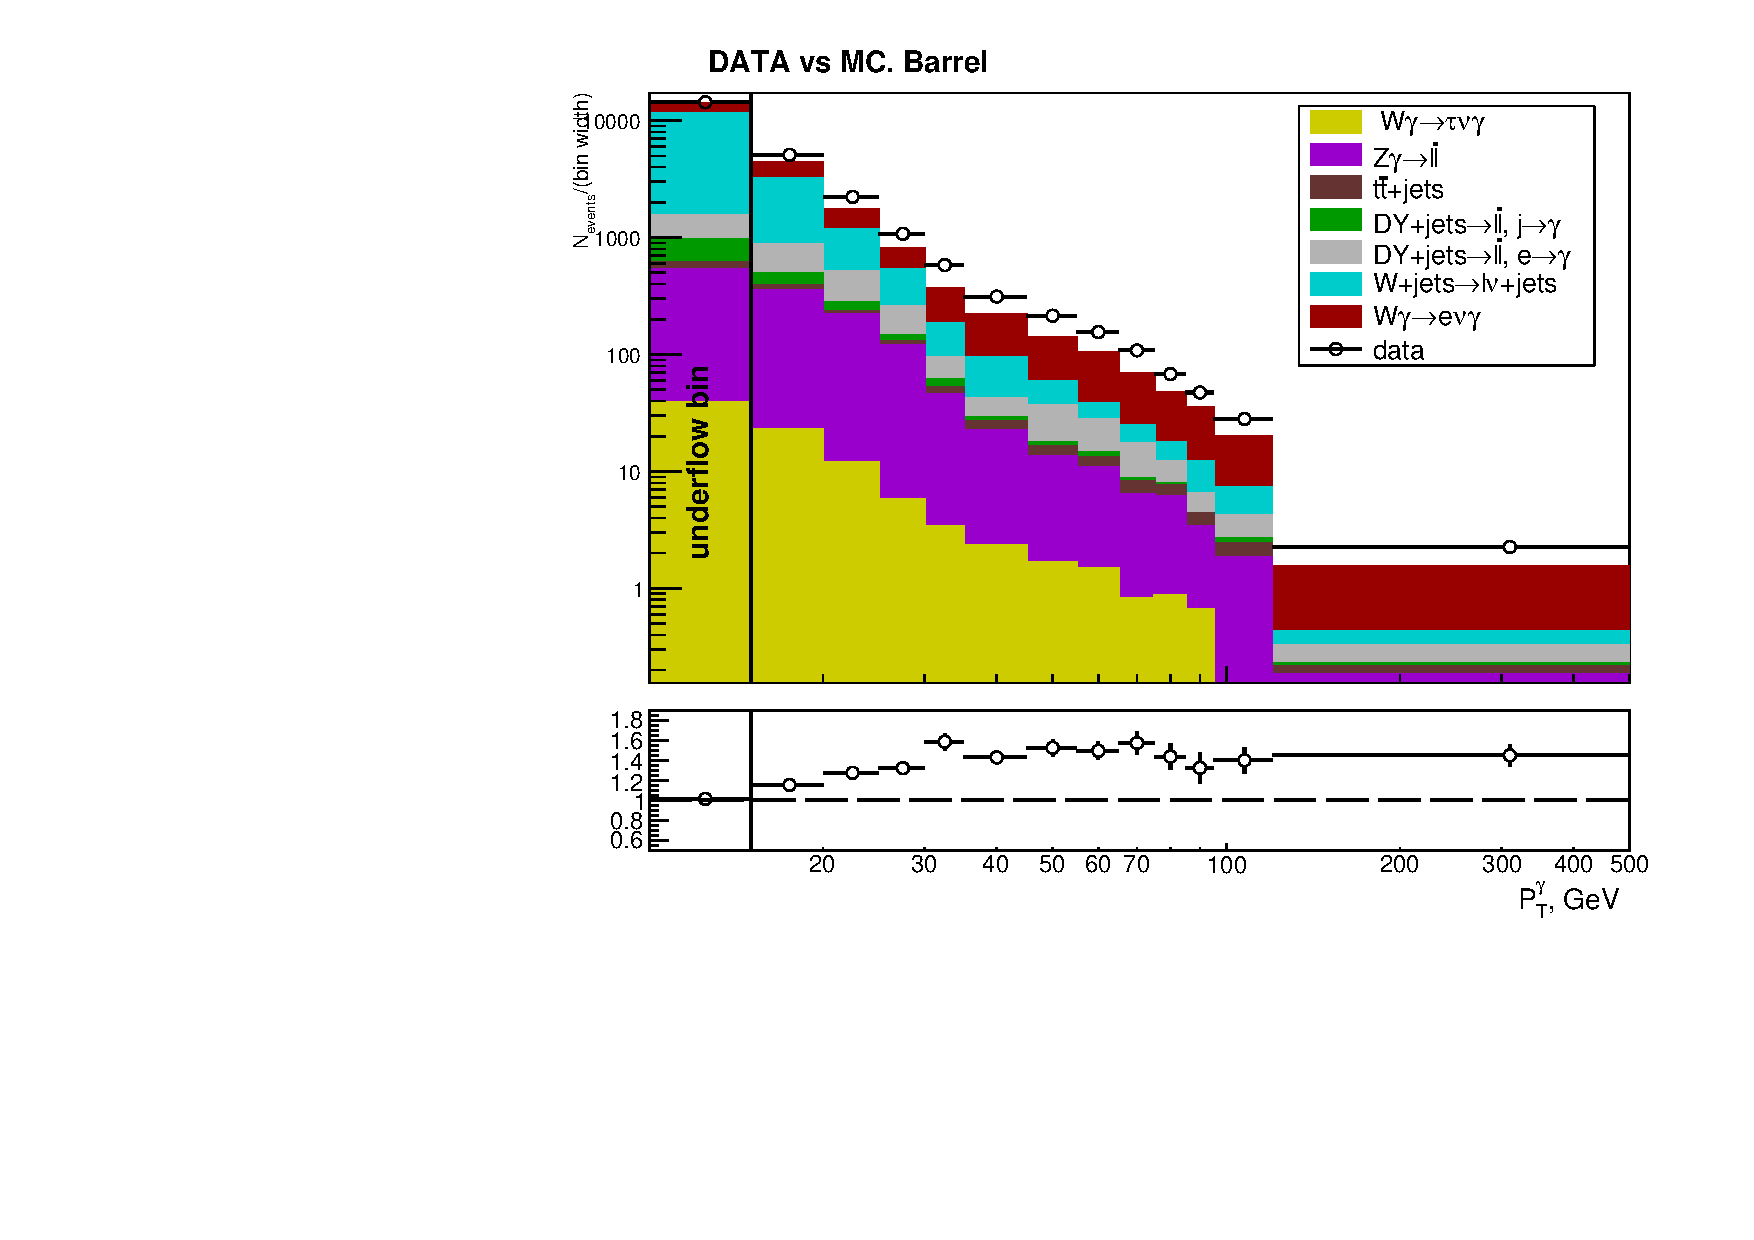
\includegraphics[width=0.49\textwidth]{../figs/figs_v11/ELECTRON_WGamma/PrepareYields/c_TotalDATAvsMC_Barrel__phoEt.pdf} 
    \end{center}
  \end{figure}
\end{frame}
